\maketitle
\section{Introduction}





In \cite{FourBall} Ozsv{\'a}th and Szab{\'o} defined a smooth concordance invariant, denoted $\tau(K)$, whose value for the $(p,q)$ torus knot provided a new proof of Milnor's famous conjecture on the unknotting number of torus knots. Rasmussen independently discovered this invariant in his thesis, \cite{Ras1}. Milnor's conjecture has a long history in gauge theory, and its original proof is due to Kronheimer and Mrowka, \cite{KM}.  Recently, however, Rasmussen \cite{Ras2} discovered another smooth concordance invariant whose value for torus knots proves the conjecture.   Denoted $s(K)$, the invariant is defined using a refinement, due to Lee \cite{Lee}, of the purely combinatorial knot (co)homology  theory introduced by Khovanov \cite{Khovanov}.  Rasmussen's proof of the Milnor conjecture using $s$ is the first proof which avoids the analytical machinery of gauge theory.  It was noted immediately that the two invariants share several formal properties (e.g. an inequality relating the invariants of knots which differ by a crossing change) which in turn imply that they agree (or more precisely, that $s(K)$ and $2\tau(K)$ agree) for many knots.  For instance, $s(K)=2\tau(K)$ for the following families of knots:

\begin{enumerate}
	\item Torus knots:  $s(K)=2\tau(K)=2g(K)$ where $g(K)$ denotes the Seifert genus of $K$. This is due to Rasmussen \cite{Ras2}  for $s$ and \ons \ \cite{Lens} for $\tau$.  
	\item Alternating knots: $s(K)=2\tau(K)=\sigma(K)$ where $\sigma(K)$ is the classical Tristam-Levine signature of $K$. This is due to Lee \cite{Lee} for $s$, and \ons \ \cite{AltKnots} for $\tau$. 
	\item Strongly quasipositive knots, in particular positive knots: $s(K)=2\tau(K)=2g(K)$.  This is due to Livingston, \cite{Livingston1}.  See also \cite{Rudolph}.
	\item Quasipositive knots: $s(K)=2\tau(K)=2g_4(K)$, where $g_4(K)$ denotes the smooth slice genus of $K$. This follows from work of Plamenevskaya \cite{Olga1} for $\tau$ and from Plamenevskaya \cite{Olga2} and Shumakovitch \cite{Shumakovitch} for $s$. See also \cite{SQPfiber}.
	\item Knots with up to $10$ crossings.  \cite{Goda,Ras1,FourBall}
	\item ``Most'' twisted Whitehead doubles of an arbitrary knot, $K$.  This is due to Livingston and Naik \cite{Livingston2}
	\item Fibered knots with $\tau(K)=g(K)$. This follows from work of the first author \cite{SQPfiber}.
\end{enumerate}

\bigskip
\noindent Indeed, it was conjectured that the two invariants always coincide:

\bigskip
\noindent{\bf Conjecture}:({\em Rasmussen} \cite{Ras2}) $s(K)=2\tau(K)$ for all knots, $K$.  
\bigskip

In light of the above list, the formal properties that the two invariants share, and several other striking connections between Khovanov's homology theory and  \os \ theory \cite{Seidel,Branched,Ciprian,Ras4}, there was justified hope that the above conjecture could be true.  However, we will demonstrate a counterexample:

\begin{theorem}
	Let $D_+(T_{2,3},2)$ denote the $2$-twisted positive Whitehead double of the right-handed trefoil knot (see Figure \ref{fig:Double}).  Then $\tau(D_+(T_{2,3},2)=0$ while $s(D_+(T_{2,3},2))=2$.  
\end{theorem}

Livingston and Naik \cite{Livingston2} calculate $\tau$ and $s$ for all but finitely many twisted Whitehead doubles of a knot, $K$, in terms of the maximal Thurston-Bennequin number of $K$, $TB(K)$, and its reflection, $\overline{K}$. In particular, they show that  $\tau(D_+(K,t))=s(D_+(K,t))/2=1$ if $t \le TB(K)$ and  $\tau(D_+(K,t))=s(D_+(K,t))/2=0$ if $t \ge -TB(\overline{K})$.  In light of an inequality satisfied by $\tau$ and $s$ under the operation of a crossing change, they define an invariant (which the results of this paper indicate is actually two invariants) $t_{\tau}(K)$ (resp. $t_s(K)$) which is the greatest integer $t$ such that $\tau(D_+(K,t))=1$ (resp. $s(D_+(K,t)=2$).  Using the techniques for the calculation above, we are able to determine $t_{\tau}(K)$ for the $(2,2n+1)$ torus knots:

\begin{theorem}
\label{thm:2n}
Let $D_+(T_{2,2n+1},t)$  denote the $t$-twisted positive Whitehead double of the the $(2,2n+1)$ knot.  Then we have:

$$ \tau(D_+(T_{2,2n+1},t))= 
\left\{\begin{array}{ll}

0  & {\text{for
 $t>2n-1$}} \\

 1 & {\text{for
 $t\le2n-1$}} \\

\end{array}
\right. $$
\end{theorem}

Thus, $t_{\tau}(T_{2,2n+1})=2n-1$.  In fact, the above knots provide further counterexamples, as was shared with us by Jake Rasmussen, who used Bar-Natan's  program \cite{BarNatan} for computing Khovanov homology to calculate $s$ for the knots in the above family which are not covered by Livingston and Naik's result.  In particular:
$$ s(D_+(T_{2,5},5))= s(D_+(T_{2,5},4))= s(D_+(T_{2,7},8))= s(D_+(T_{2,7},7))= s(D_+(T_{2,7},6))=2, $$
\noindent while Theorem \ref{thm:2n} implies that $\tau=0$ for these knots.  It seems likely that Whitehead doubles of the $(2,2n+1)$ torus knots provide an infinite family of counterexamples.  Indeed, it would be reasonable to guess that $t_s(T_{2,2n+1})=3n-1$




\begin{figure}
\begin{center}

%\psfrag{t-3}{$t-3$}	
\caption{\label{fig:Double}
The $t$-twisted positive Whitehead double of the right-handed trefoil.  The box indicates the number of full right-handed twists to insert.}
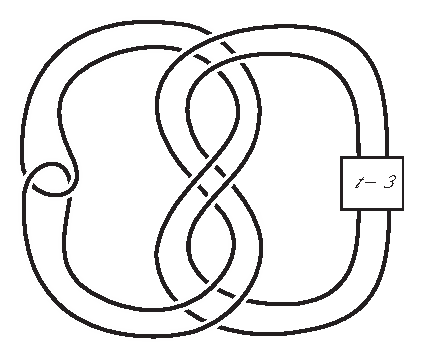
\includegraphics{twistedWD.eps}
\end{center}
\end{figure}

We prove the above results first by calculating the knot Floer homology groups of a specific twisted Whitehead double which happens to be a $(1,1)$ knot. A general technique for calculating the Floer homology of such knots was developed by Goda, Morifuji, and Matsuda \cite{Goda} and we apply their technique here.  We then use results of Eftekhary \cite{Eaman} for the $0$-twisted Whitehead double of  $T_{2,2n+1}$, together with properties of the skein exact sequence for knot Floer homology to calculate $\tau$ for the examples above.  The techniques here will be refined and generalized in \cite{Doubling} to calculate $\tau$ and some of the Floer homology of an arbitrarily twisted Whitehead double of an arbitrary knot (in fact, \cite{Doubling} will prove that $t_{\tau}(K)=2\tau(K)-1$).  We also remark that $(1,1)$ satellite knots were classified by Morimoto and Sakuma in \cite{Morimoto}, and it was in the context of a more general study of these knots that this work arose.   We hope to return to this study (see also \cite{PhilThesis}).

	We conclude by remarking that there is a beautiful conjectural picture  due to Dunfield, Gukov, and Rasmussen, \cite{Dunfield} of a triply graded homology theory which would unify Khovanov homology, knot Floer homology, and the various $sl(n)$ link homology theories of Khovanov and Rozansky \cite{Khovanov2}.  It would be very interesting to understand this conjecture for the above examples - in particular it would be useful to calculate the $sl(n)$ link homology.
	
	\noindent{\bf{Acknowledgements:}} It is our pleasure to thank  Hiroshi Goda, Hiroshi Matsuda, Peter Ozsv{\'a}th, Zoltan Szab{\'o}, and Jake Rasmussen for many stimulating discussions.  We owe special thanks to Jake for computing $s$ for the examples in this paper and for sharing both his results and his general knowledge of the $s$ invariant with us. 

